\chapter{Far Out Memory Hierarchies}\label{ch:farout}

\squo{“I never am really satisfied that I understand anything; because, understand it well as I may, my comprehension can
    only be an infinitesimal fraction of all I want to understand about the many connections and relations which occur
    to me, how the matter in question was first thought of or arrived at…”
}
{Ada Lovelace}

\begin{chabstract}
    The world is changing around us!
    This chapter introduces the hardware trends that we observe and discusses some of the details behind our expectations of how these trends will pan out. We will discuss persistence,
    including both SSDs and NVM, along with memory disaggregation, interconnect technologies, and device controller complexity.
\end{chabstract}

Operating systems provide abstractions for data access that reflect the hardware for which they are designed. For example, our current I/O interfaces reflect a structure that takes as axiom
the separation between volatile and persistent data domains. Any assumptions we make about hardware, however, may become less accurate over time, resulting in an increasing impedance mismatch
between the interfaces provided and the underlying hardware.

\squo{One of the most basic goals is to build up some abstractions in order
    to make the system convenient and easy to use. Abstractions are fundamental to everything we do in computer science. Abstraction makes
    it possible to write a large program by dividing it into small and understandable pieces [...] Abstraction is so fundamental that
    sometimes we forget its importance.}{Operating Systems: Three Easy Pieces~\cite{ostep}}


It therefore pays to examine the trends in hardware\sidenote{And software, as we will see in the next chapter.} and reexamine how we expose that hardware to applications. The work presented
herein starts with the assumption that hardware trends are, at minimum, worth examining to see how we may wish to update our interfaces. We argue further that the trends and
opportunities we are presented with demand a full scale revolution in how programming models are designed, and in the design of operating systems that wish to support new models. Let's
first explore some hardware trends, and then, in the next chapter, put those trends in the context of the software that we wish to better support.


\section{Memory and Compute}

Memory and storage are getting closer \emph{and} further away\sidenote{Bear with me, now!}. Closeness of memory to CPU in latency space has long been a vital part of ensuring speedy
computation. However, in the constant battle between latency and throughput (and complexity and density), latency often
loses, and the latencies of DRAM have not seen dramatic reductions
for some time. Meanwhile, access to \emph{persistent} memory is getting faster---both in latency \emph{and} throughput.
Not only are SSDs constantly improving, but so too are the protocols they use and the link speeds between them and main
memory~\cite{xu:systor15,lee:atc19}.

Recently, we have also seen commercially available byte-addressable NVM
%\sidenote{This document will use the acronym NVM to refer to low-latency, directly attached non-volatile
%    memory. If I want to talk about SSDs, I will be explicit.}
in a DIMM form-factor. This technology, Intel Optane\sidenote{We will discuss the outcome of Intel's
    ``attempt'' to market this technology later.} (using 3D-Xpoint technology), provides a persistent memory
with low latency---only $1.5$--$8\times$ the latency of DRAM in most cases~\cite{ucsd_bnvm}---that is accessible from the CPU directly via normal load/store instructions. Direct, low latency
access to NVM opens the door to building the system around persistent data structures and avoiding serialization\sidenote{Indeed, this is what we will do.}.

We can view the emergence of NVM as an extreme example of the general trend of persistence getting closer to compute. As a result, the relative cost of indirection and kernel involvement in
the data path is increasing. While before the cost of a system call was significantly less than that of the actual device activity, now we are seeing the cost of device access shrinking to a
similar magnitude of the cost of a system call, or in the case of \NVM, even less.

\subsection{Distribution}

However, to stop here would be a mistake. Another significant trend is \emph{disaggregation}, in which memory is placed across machines and programs are written expecting various levels of
access to this distributed memory. This is, admittedly, as much about software as it is about hardware, however there are underlying hardware mechanisms that are driving the push toward
decoupling memory and compute. On a network level, renewed interest in \ac{dsm} is sourced from a combination of several factors:

\begin{enumerate}
    \item Network speeds are increasing. With technologies like 100 Gig NICs and 10 Tb/s switches, previous limitations on distributed memory sourced from network performance reduce or go away entirely.
    \item Network hardware complexity is increasing. Not only can those switches sustain 10 Tb/s throughput, but they can be programmable, allowing the network much more participation in
          protocols. Furthermore, we are seeing protocols like RDMA enabling remote memory access via the network.
\end{enumerate}

It isn't just traditional networking in which memory semantics are leaking out past a single traditional node. Interconnect technologies like CXL have the potential to upend the
traditional view of ``CPU attached to memory with peripheral devices'' as the fundamental concept of a node. These trends mirror the persistence trends above---things that were traditionally far away (other nodes' memories) are getting closer in a logical space, and
things that were close (local DRAM and storage) can be more efficiently shared.

Finally, improved fabrication techniques and shrinking feature
sizes means hardware controllers are increasing in complexity, offering more autonomy from the CPU,
off-CPU processing capabilities, and better parallelism. Hardware interfaces reflect the controller
complexity expected of devices; for example, AHCI controllers improved request queuing over ATA, and DMA
allows hardware to copy data directly to and from memory independent from the CPU. NVMe
expands the responsibility of controllers again, adding deeper and parallel command queues, requiring
devices to multiplex requests themselves and allowing them to exploit the parallelism of access
available in SSDs. We expect these trends to continue, resulting in more programmable hardware
devices that are able to act on shared, global memory with more autonomy.

\subsection{Memory Density}

Another point to make is one of increasing memory sizes, largely stemming from increased density of memory technology.
Not only can we see this in DRAM, with well-known systems taking advantage of
increased DRAM sizes~\cite{ousterhout15}, one of the major selling points of Intel's Optane NVM was a significant
increased density and lower cost per byte. Having larger memories means a few things:

\begin{enumerate}
    \item Some nodes may have wasted memory as workloads come and go. This ties in with the above points about
          disaggregated memory---sharing unused memory is more cost effective, since unused RAM is wasted RAM.
    \item Memory can have an induced-demand effect. Similar to how building additional lanes on highways often just increases
          traffic~\cite{traffic}, making more memory available can cause additional memory traffic since working sets can be larger.
    \item In-memory sharing can increase. With significantly larger memories, applications can take advantage by not
          writing intermediate results to storage, and instead can write to shared memory.
\end{enumerate}

\subsection{The Heterogeneity of Memory}

The advent of NVM in a DIMM form factor has given us further motivation to consider the effects of a heterogeneous
memory environment. When all memory is a single ``kind'' (\eg DRAM), it matters little from where in the physical
address space memory is allocated, since devices (including the CPU) can only access one kind of memory between
them\sidenote{Yes, older devices are limited in address space, but this is not important, and I do not wish to get stuck
    in the past.}. However, if our physical memory is comprised of multiple kinds of memory, we must be more careful with
our allocation. Programs may request allocations of memory for their data based on different policies of what kind of
memory they want---volatile versus persistent, high-bandwidth versus DRAM, to name a few.

But it's not just allocation policy that is affected. Having different kinds of memory means that large-scale movement
of data between regions of physical memory is now semantically meaningful and may be triggered as a result of policy,
evictions, \etc. Interacting devices, therefore, must coordinate on a shared mapping of logical data to physical data,
as the physical data might move between kinds of memory. One could easily argue that this heterogeneity is not actually
new---with NUMA, we see many of the same problems. I agree! However, the correct solution is to design around a
fundamentally heterogeneous memory system and build the concepts of data movement across physical
memory into the core abstractions. Such a model is not only useful for the advent of NVM on the memory bus, but future additions of different kinds
of memory as well.

\section{Some Kind of Model}
\begin{SCfigure}
    \centering
    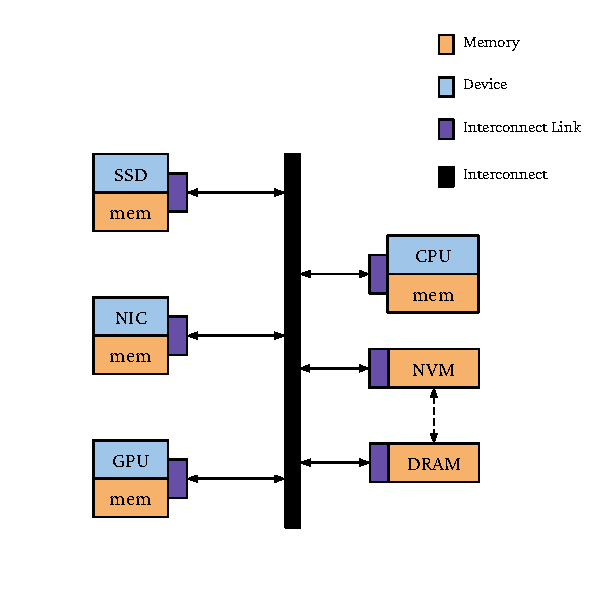
\includegraphics[width=\linewidth]{fig/gen_sys_diag}
    \caption[Expected hardware system architecture]{Our expected system architecture. Solid black lines indicate data paths. Dashed lines and boxes indicate potential dedicated paths.}
    \label{fig:sys_arch}
\end{SCfigure}


These changes are coupled with a shift in focus for how data moves throughout the system.
Traditionally, data is considered to move into main memory for computation by the CPU, followed by
storage to persistent memory (through a disk or SSD controller) or moved out onto the network
(through a network controller). Figure~\ref{fig:sys_arch} shows a different model, where data is able to more
fluidly move
through the system, or even needs less movement. With more complex controllers and off-CPU processing, we expect
non-traditional data paths to become more common. Say, for example, a packet arrives at the NIC
containing compressed data for GPU processing. A traditional system would move the compressed data
into main memory, decompress it using the CPU, and move it into GPU memory for processing. Instead,
we could see a dedicated compression chip in the NIC whose job it is to decompress incoming data.
That data could then be moved directly between the NIC's buffers and the GPU memory, without involving
the CPU and main memory at all. This both reduces copies and frees these
resources for other uses.

Note the rather generic model in Figure~\ref{fig:sys_arch}. We are intentionally not ascribing specific properties to
the components protrayed within. Attemping to build generic system abstractions atop an abstracted model while not
losing too much in the abstraction is a fundamental essence of operating system design. Here, we are trying to capture
the basic ideas of the trends we discussed---individual, higher powered devices, accessing shared memory pools and
possibly each others' memory pools, with possible NVM and fast interconnects that allow addressing control and
isolation\sidenote{Cache coherence is an issue that we are not explicitly designing for or against. It remains to be
    seen how cache coherence between these devices will play out. Nonetheless, the issues of coherence and failure-atomicity
    are not lost on us, and we will discuss them in Chapter~\ref{ch:prog}.}. Concretely, we can see this model mapping well to, for example, CXL, and even current PCIe systems\sidenote{If we squint
    our eyes
    and have perhaps undue faith in the IOMMU.}. As the trends we observe continue, the inherent concurrency enabled by
allowing devices to operate more independently with more ability to share memory without waiting for permission from the
CPU and the reduced lengths of code paths in processing data points strongly to a model like the one we describe here.

\begin{chconc}[So, What Does This All Mean?]

    The trends above imply several basic requirements for a set of operating system interfaces:

    \paragraph{Remove the kernel from the data access path} The cost of system calls is too large relative to device
    access to justify their use in the data path. We must provide lightweight, direct, memory-style access for
    programs to operate on data.
    %% TODO expand this

    \paragraph{Assume data lifetime is disconnected from ephemera} Memory can now be pooled in units outside the
    purview of the CPU. This can happen either in time---data can be persisted, where the CPU loses control over that
    data when power is cycled---or in space---where data can traverse a network, be accessed by
    multiple devices on an interconnect. While these forms of temporal and spacial sharing have always existed, they
    have either been relegated to ``experts'' in cordoned off low-level areas of the system (drivers and DMA) or have
    been explicitly designed around by, for example, building OS abstractions around an assumed bifurcation of data into
    ``volatile'' and ``persistent'' domains, and asking programmers to explicitly move data between
    them\sidenote{We will explore this more fully in the next chapter.}.

    However, when the previously outcast
    domains of persistence and network become closer to compute as we saw above, either via faster access or pushing compute power
    further out, we must \textbf{design for in-memory data structures}. Long-lived data structures can directly reference
    persistent data, so references must have the same lifetime as the data they point to. Virtual memory mappings are, by
    contrast, ephemeral, and so cannot effectively name persistent or distributed data. But perhaps more importantly,
    in-memory data structures are \emph{what we compute on}, and it's \emph{computation} that matters most. If we can reduce
    or even remove extraneous processing paths that waste time, we should take that opportunity.


    \paragraph{Towards a Data-Centric Operating System}
    We call an operating system that meets both of the above requirements
    \emph{data-centric}, as opposed to current OSes, which are \emph{process-centric}.
    Facilitating
    operations by applications on in-memory data structures is the primary function of a data-centric OS,
    which tries to avoid interposing on such operations, preferring instead to intervene only when
    necessary to ensure properties such as security and isolation. To meet both of these requirements
    a data-centric OS must provide effective abstractions for identifying data independent
    of data location, constructing persistent and distributed data relationships that do not depend on ephemeral
    context, and facilitating sharing and protection.



    %% This section will discuss the trends of moving persistence closer to computation, or moving
    %computation closer to persistence. Key points: memory lifetime, and removing the kernel from data
    %path (more broadly, facilitating direct access to persistent data and reducing the lengths of code paths).



    %\section{Memory Distribution}

    % This section will cover how memory semantics are spreading out, with things like RDMA and CXL. Key
    % points: memory semantics spreading out, but having to keep tabs on latency. From another
    % perspective, this is disaggregated computing. Want to avoid costs that increase code path length.

    %\section{Memory Capacity}

    % This section will discuss the increasing size of memory (both from DRAM and NVM). Key points:
    % memory cost and power, larger memory means more in-memory sharing.

    %\section{Increasing Hardware Complexity and Performance}

    % This section argues that controllers are increasing in complexity and offload capabilities. Thus
    % we are getting closer and closer to treating a single node as a distributed system. Additionally,
    % increasing interconnect speeds make memory distribution easier, and things like
    % paxos-in-the-switch can improve coordination at-scale.

    \paragraph{Why Now?}

    %\todo[inline]{This will take some strong arumentation.}

    %It is natural at this point to wonder, ``why now? The memory hierarchy has \emph{always} been changing.'' This is true,
    %dear reader---indeed, where \emph{was} Gondor when the Westfold fell? And where \emph{is} Gandalf, for I \emph{much}
    %desire to speak with him.

    It is natural at this point to wonder, ``why now? The memory hierarchy has \emph{always} been changing.'' This is true,
    but there are a few unique elements to the recent changes we are seeing. First, the placement of NVM directly on the
    memory bus is a fundamental dramatic shift in how we view persistence and opens the door to \emph{true} single-level
    stores. Second, the increasing distribution of both memory and CPU requires that we rethink how computation is delegated
    throughout the system and how those separate memories and devices can organize, access, and reference data.
    But, more fundamentally, this thesis argues that our data-centric model was \emph{always} the correct model. We just
    have an opportunity to realize it, and modern hardware has the ability to make it efficient and scalable. The memory
    hierarchy has always been changing, but our interfaces have not kept pace. It is time for a revolution, designed for
    upcoming hardware and, as we'll see in the next chapter, informed by software.

    %% TODO add: it's a good time, lots of renewed interest, OS research is popping off

\end{chconc}

\iffalse
    \begin{chconc}
        This chapter covered the core hardware trends we are concerned with: faster persistent memory, faster and more flexible
        interconnects, larger memories, and more interest in distributed memory and compute. These trends point to a
        fundamental shift towards a \emph{data-centric} model, in which the data's the thing, and enabling efficient
        computation is the central goal. To this end, the OS has to get out of the way and we need to minimize code paths
        surrounding the computation that just waste time. The next chapter will put these ideas into context for what
        software is demanding from hardware and from interfaces.
    \end{chconc}
\fi